% Created 2018-09-07 Fri 08:32
% Intended LaTeX compiler: pdflatex
\documentclass[presentation]{beamer}
\usepackage[utf8]{inputenc}
\usepackage[T1]{fontenc}
\usepackage{graphicx}
\usepackage{grffile}
\usepackage{longtable}
\usepackage{wrapfig}
\usepackage{rotating}
\usepackage[normalem]{ulem}
\usepackage{amsmath}
\usepackage{textcomp}
\usepackage{amssymb}
\usepackage{capt-of}
\usepackage{natbib}
\usepackage[linktocpage,pdfstartview=FitH,colorlinks,
linkcolor=blue,anchorcolor=blue,
citecolor=blue,filecolor=blue,menucolor=blue,urlcolor=blue]{hyperref}
\setbeamertemplate{frame footer}{\insertshortauthor}
\setbeamerfont{page number in head/foot}{size=\tiny}
\setbeamercolor{footline}{fg=gray}
\author{Florian Hollenbach}
\usepackage[english]{isodate}
\usepackage{amsmath,amsthm,amssymb,amsfonts}
\usetheme{metropolis}
\usecolortheme{}
\usefonttheme{}
\useinnertheme{}
\useoutertheme{}
\author{Florian Hollenbach}
\date{\today}
\title{Political Science 209 - Fall 2018}
\subtitle{Causal Inference}

\hypersetup{
 pdfauthor={Florian Hollenbach},
 pdftitle={Political Science 209 - Fall 2018},
 pdfkeywords={},
 pdfsubject={},
 pdfcreator={Emacs 25.3.1 (Org mode 9.1.9)}, 
 pdflang={English}}
\begin{document}

\maketitle


\begin{frame}[label={sec:org2391538}]{Causal Inference}
\begin{block}{What do you think is causal inference?}
\end{block}
\end{frame}

\begin{frame}[label={sec:orgec246e6}]{Causal Inference}
\begin{itemize}
\item causal: relationship between things where one causes the other
\item inference: to derive as a conclusion from facts or premises
\end{itemize}

Causal inference is the \uline{\uline{attempt}} to derive causal connection based on the conditions of the occurrence of an effect
\end{frame}

\begin{frame}[label={sec:org911941f}]{Causal Inference}
\begin{itemize}
\item Most questions that empirical (political) scientist are interested in are causal questions
\end{itemize}
\end{frame}

\begin{frame}[label={sec:orge8856a2}]{Causal Inference}
\begin{block}{Examples from Political Science}
\begin{center}
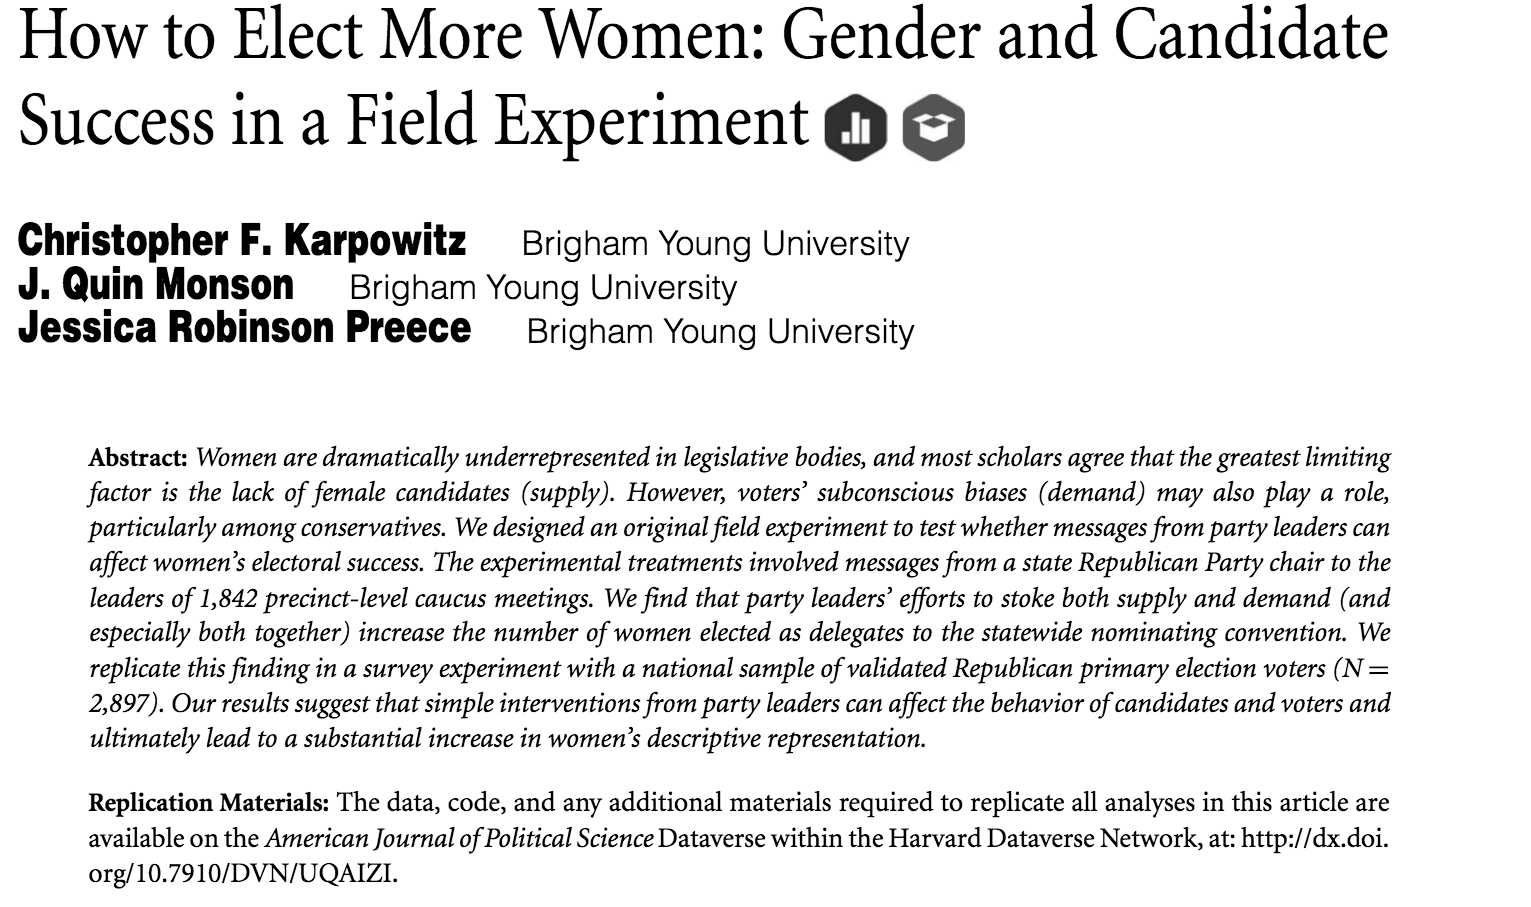
\includegraphics[width=8cm]{/Users/florianhollenbach/Documents/GitHub/Polisci209_2018/slides/week2/experiment1.png}
\end{center}
\end{block}
\end{frame}

\begin{frame}[label={sec:orgf0b6048}]{Causal Inference}
\begin{block}{Examples from Political Science}
\begin{center}
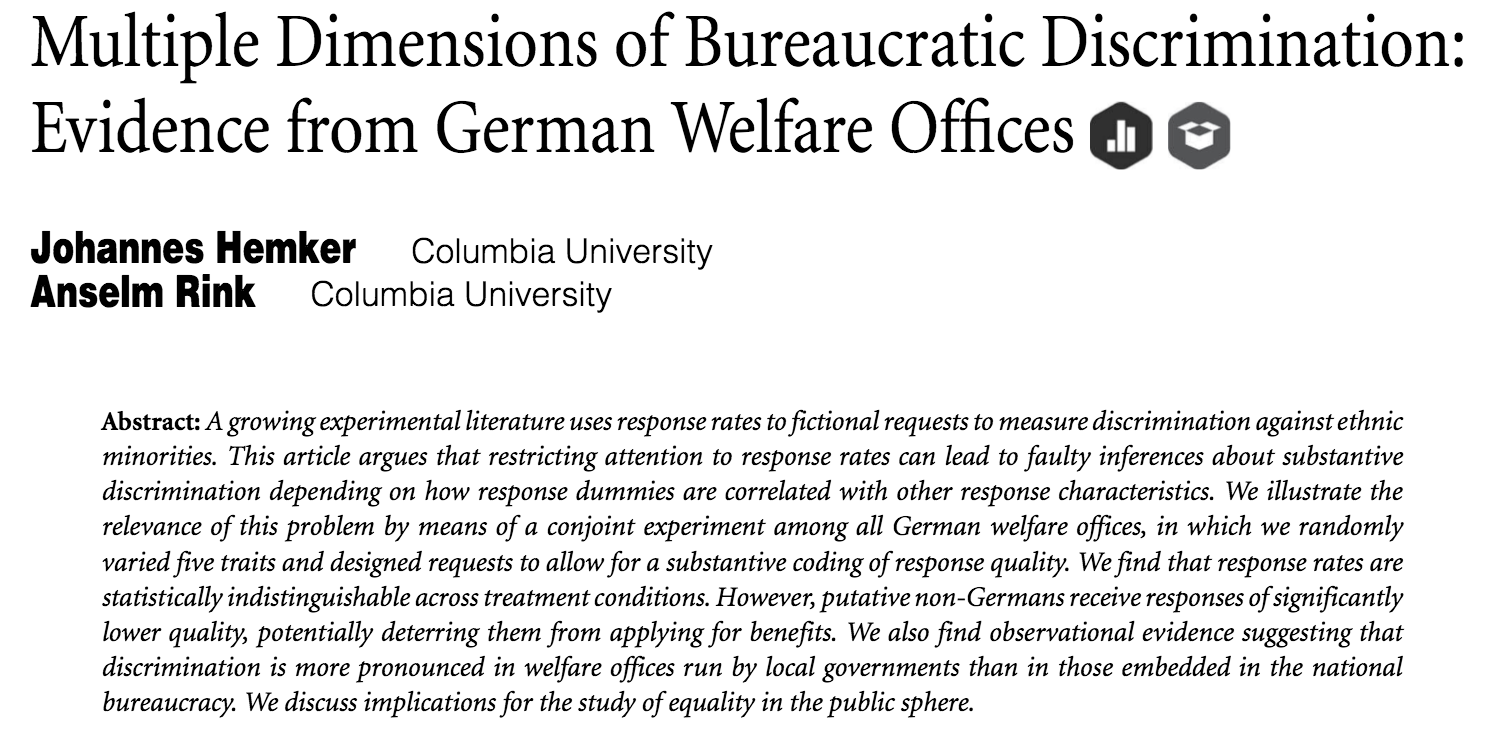
\includegraphics[width=8cm]{/Users/florianhollenbach/Documents/GitHub/Polisci209_2018/slides/week2/experiment2.png}
\end{center}
\end{block}
\end{frame}

\begin{frame}[label={sec:org791652e}]{Causal Inference}
\begin{block}{Examples from Political Science}
\begin{center}
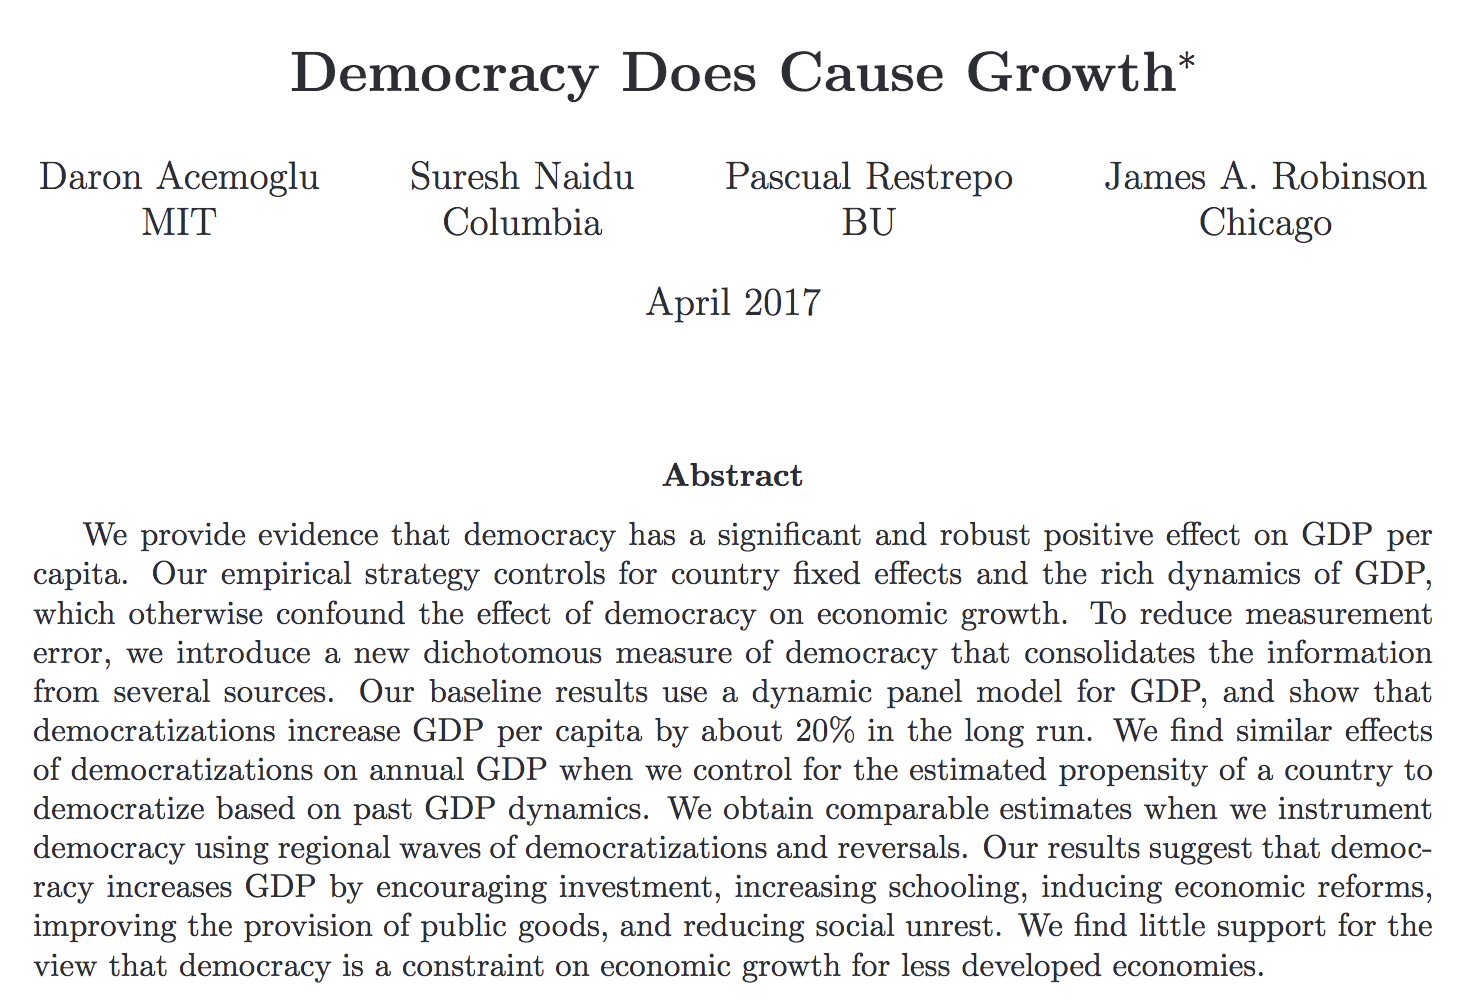
\includegraphics[width=8cm]{/Users/florianhollenbach/Documents/GitHub/Polisci209_2018/slides/week2/democracy.png}
\end{center}
\end{block}
\end{frame}

\begin{frame}[label={sec:org9eb7711}]{Causal Inference}
Do you think one of these questions is harder to answer than the others?
\end{frame}

\begin{frame}[label={sec:orgb1f2eb1}]{Causal Inference}
Think of the causal effect as the difference between what happened and what could have happened with/without a \emph{treatment} (or change in X)

\emph{How do we measure the causal effect?}
\end{frame}

\begin{frame}[label={sec:org60b8f82}]{Is there a causal effect of democracy on child mortality?}
\begin{center}
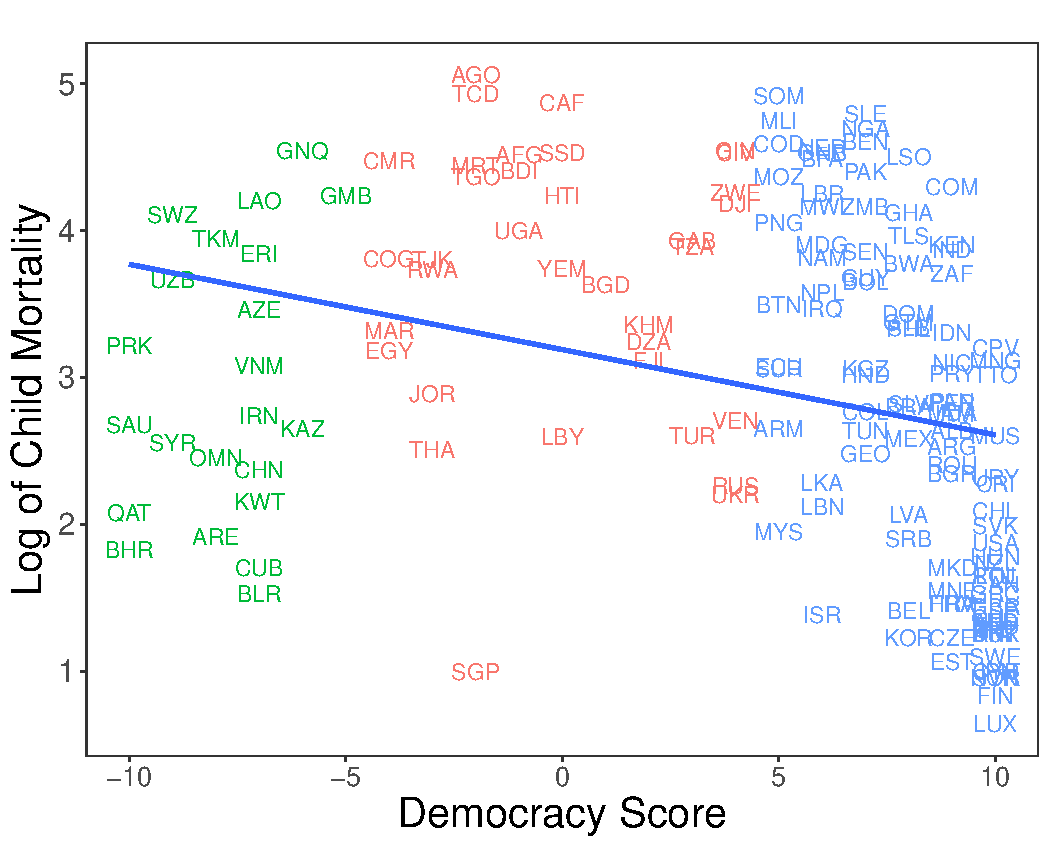
\includegraphics[width=8cm]{/Users/florianhollenbach/Documents/GitHub/Polisci209_2018/slides/week2/mortalitydemocracy.pdf}
\end{center}
\end{frame}

\begin{frame}[label={sec:org5b1ea32}]{Is there a causal effect of democracy on child mortality?}
\begin{center}
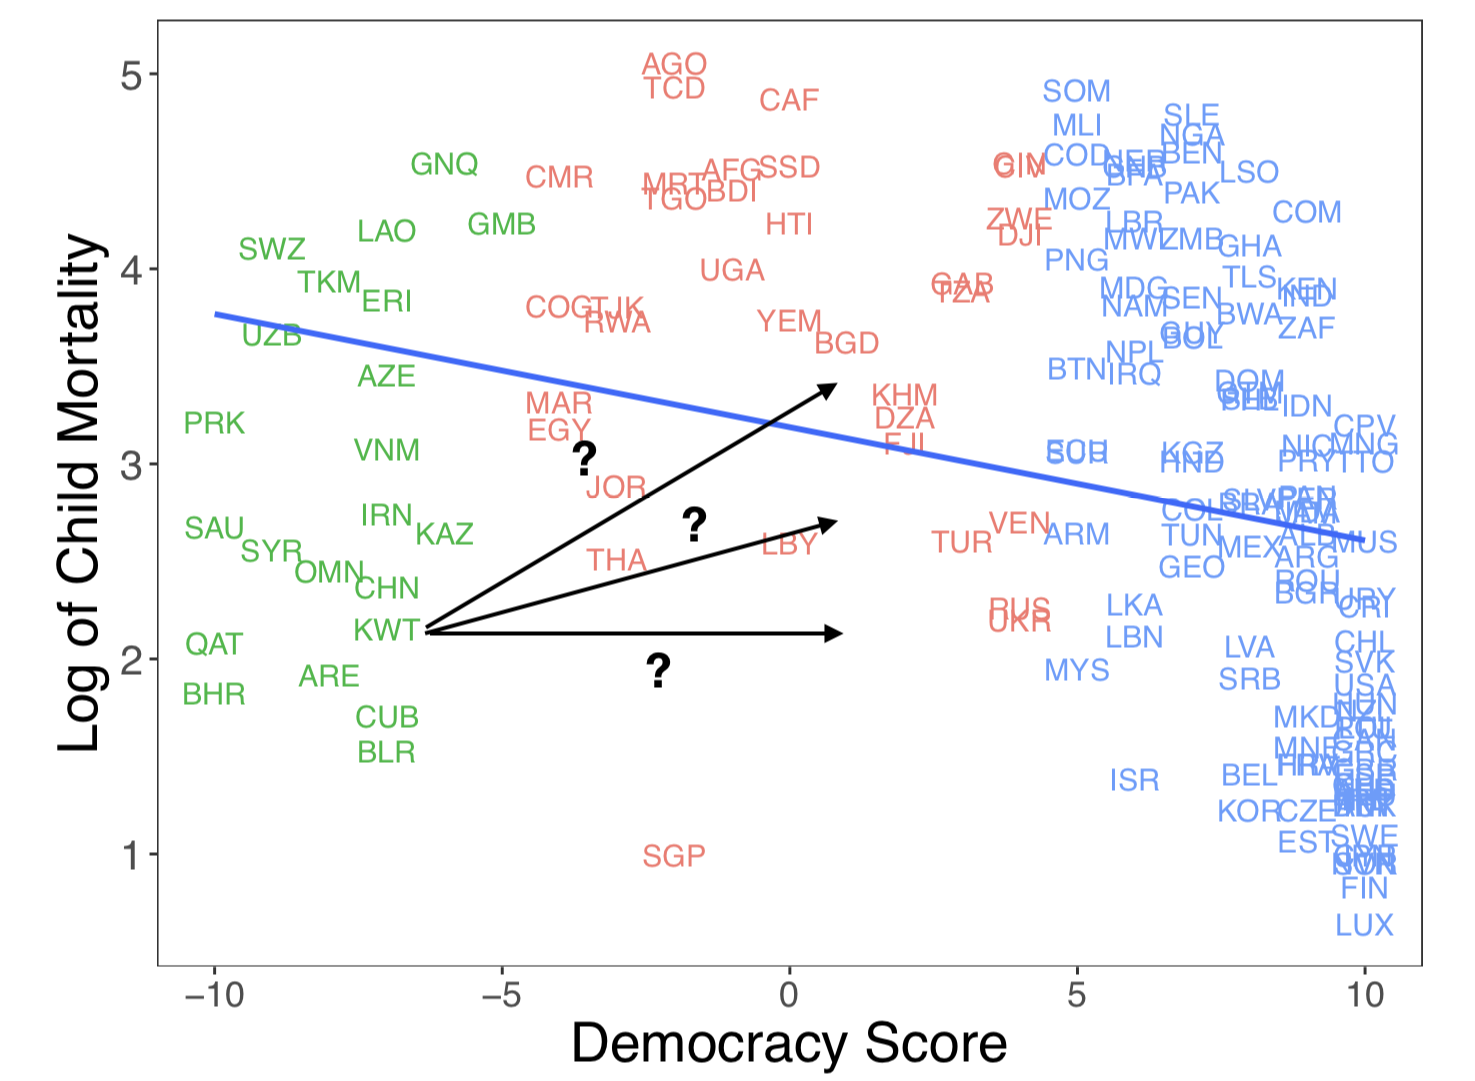
\includegraphics[width=8cm]{/Users/florianhollenbach/Documents/GitHub/Polisci209_2018/slides/week2/mortalitydemocracy2.png}
\end{center}
\begin{block}{What if Kuwait was more democratic?}
\end{block}
\end{frame}

\begin{frame}[label={sec:orgd1c4bf3}]{How would you know if two variables are causally related?}
\LARGE{X $\rightarrow$ Y ?}

\pause
\LARGE{T $\rightarrow$ Y ?}
\end{frame}


\begin{frame}[label={sec:orgbe7b179}]{How would you know if two variables are causally related?}
\Large{How would you know if two variables are causally related?}
\end{frame}


\begin{frame}[label={sec:orgb934b50}]{How would you know if two variables are causally related?}
\begin{itemize}
\item they occurr together?
\item if X goes up, Y goes up
\item if X happens, Y happens
\item if T, then change in Y
\end{itemize}


\pause
If two things happen together a lot, we say they are correlated
\end{frame}

\begin{frame}[label={sec:org5b6d5fa}]{Is correlation sufficient for causation?}
\Large{Is correlation sufficient for causation?}
\end{frame}

\begin{frame}[label={sec:orgdacefdf}]{Is correlation sufficient for causation?}
\LARGE{NO}
\end{frame}

\begin{frame}[label={sec:orgdcac148}]{Is correlation sufficient for causation?}
\LARGE{NO}

\begin{center}
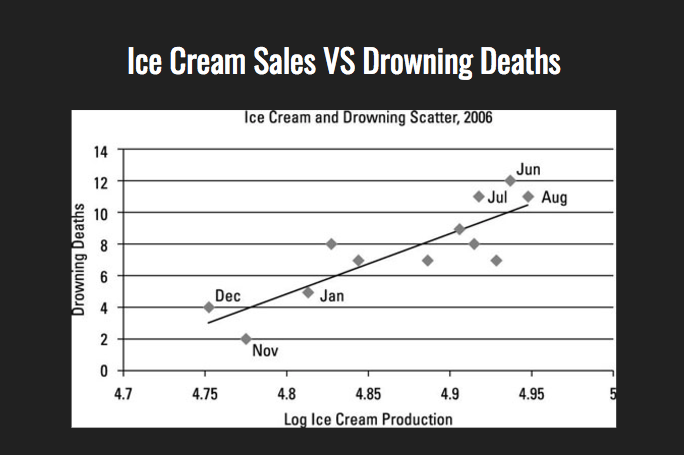
\includegraphics[width=8cm]{/Users/florianhollenbach/Documents/GitHub/Polisci209_2018/slides/week2/icecream.png}
\end{center}
\end{frame}


\begin{frame}[label={sec:org0bdc31e}]{Is correlation sufficient for causation?}
\LARGE{NO}

\begin{center}
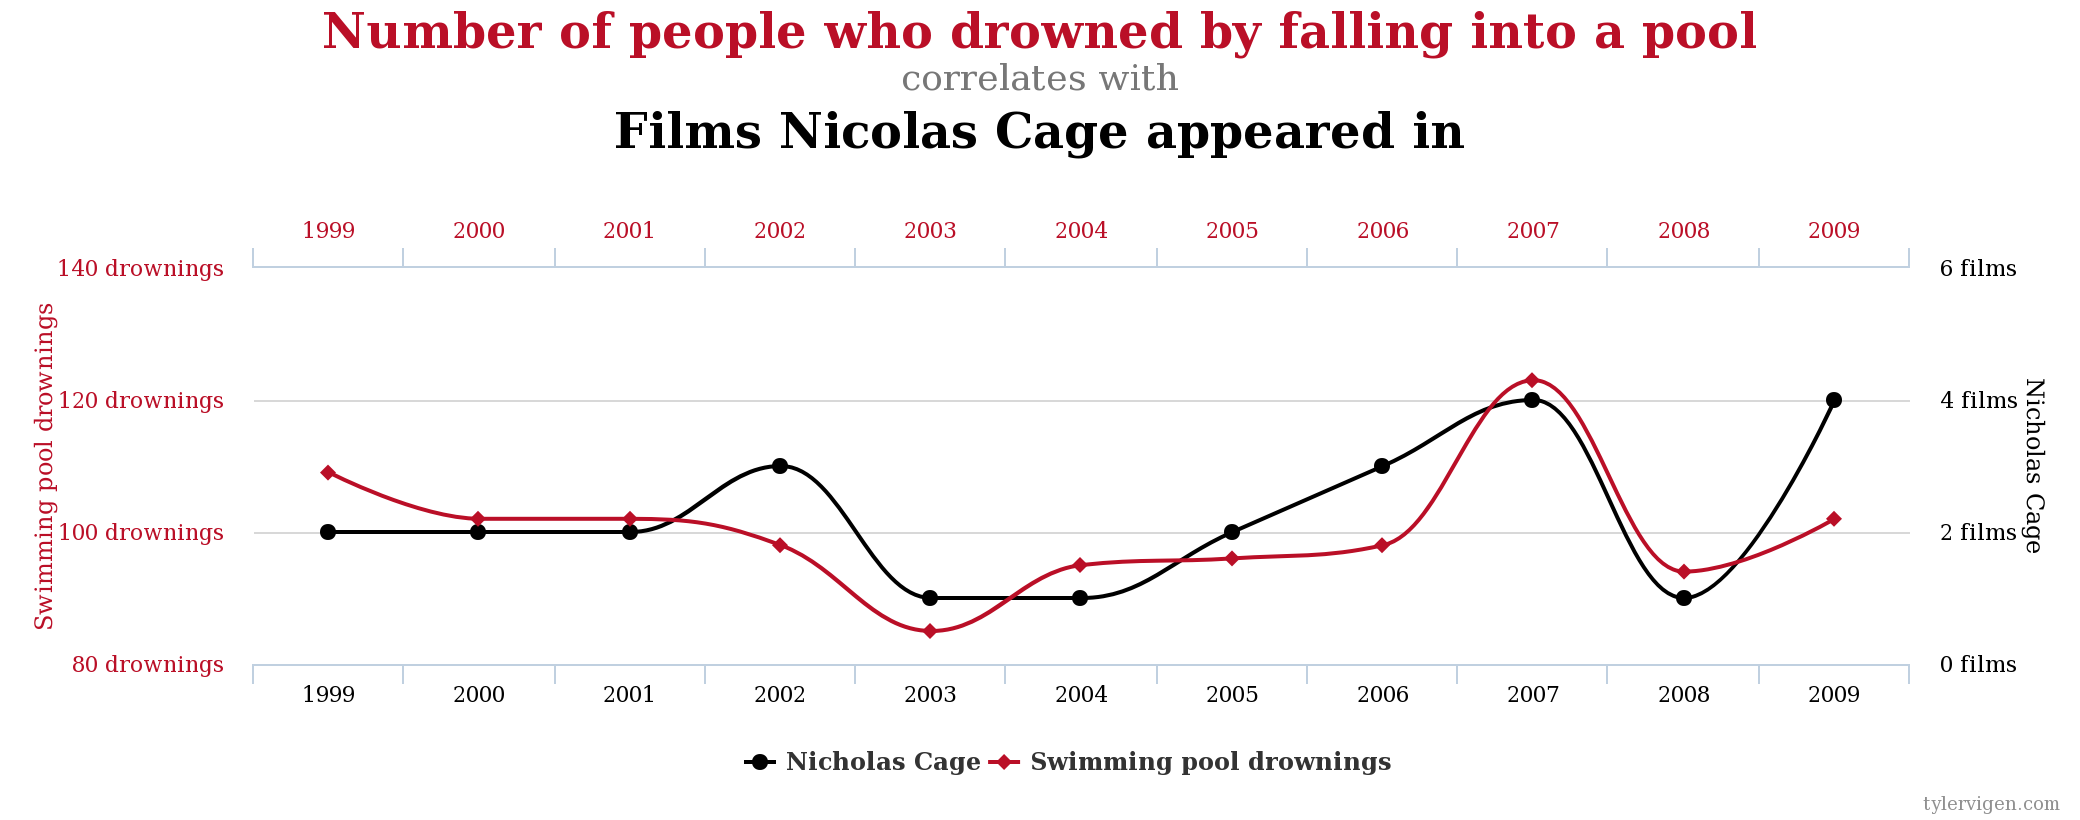
\includegraphics[width=8cm]{/Users/florianhollenbach/Documents/GitHub/Polisci209_2018/slides/week2/chart.png}
\end{center}
\end{frame}



\begin{frame}[label={sec:org0adce73}]{Causal Inference - Concepts}
\begin{itemize}
\item Key causal variable: \emph{Treatment (T)}
\item Two \emph{potential outcomes}: Y with T = 0 and Y with T = 1
\end{itemize}

\pause
Example:
\begin{itemize}
\item \emph{Treatment}: getting BS in political science instead of BA
\item \emph{potential outcomes}: Salary after getting BS (Y (T = 1)) or after BA (Y (T = 0))
\end{itemize}
\end{frame}


\begin{frame}[label={sec:org192503f}]{Why is causal inference so hard?}
\begin{itemize}
\item The causal effect of a \emph{treatment} is the difference in the \emph{outcome} with and without the treatment:
Y(T = 1) - Y(T = 0) \(\rightarrow\) Y(1) - Y(0)
\end{itemize}

\pause
\begin{center}
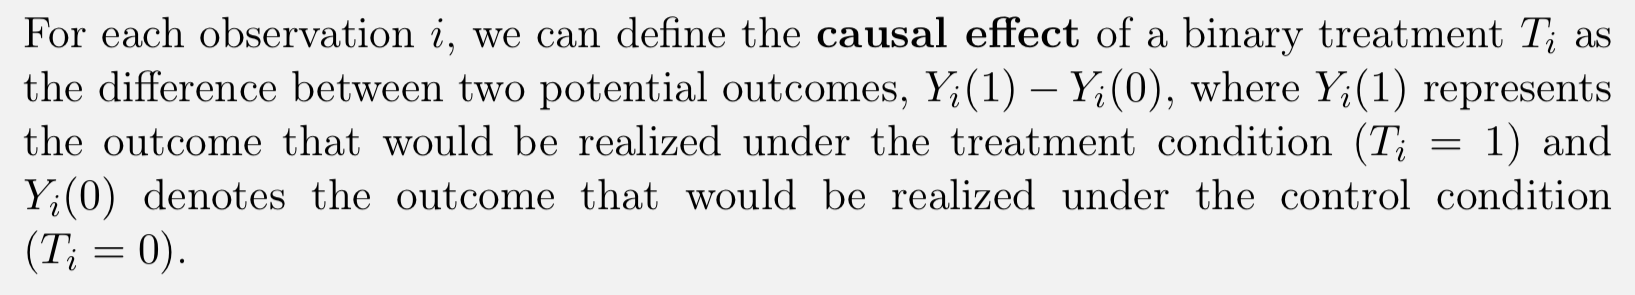
\includegraphics[width=10cm]{/Users/florianhollenbach/Documents/GitHub/Polisci209_2018/slides/week2/causaleffect.png}
\end{center}

\begin{itemize}
\item Why might this be a problem?
\end{itemize}
\end{frame}

\begin{frame}[label={sec:org98968d7}]{Fundamental Problem of Causal Inference}
We never observe the \emph{counterfactual}, i.e. the outcome if the \emph{treatment condition} was different

\pause
Example:
\begin{itemize}
\item \emph{Treatment}: getting BS in political science instead of BA
\item \emph{Potential outcomes}: Salary after getting BS (Y (T = 1)) or after BA (Y (T = 0))
\item For each of you we only observe one outcome
\end{itemize}
\end{frame}


\begin{frame}[label={sec:orga730eb6}]{Fundamental Problem of Causal Inference}
Examples:

\begin{itemize}
\item We don't observe Kuwait as a democracy
\item You don't know how you would feel if you didn't drink that coffee
\item We don't know how the world/US would look if Clinton had won the election
\end{itemize}
\end{frame}



\begin{frame}[label={sec:org7b62b5f}]{Interlude}
\Large{What is College about?}

\pause
\begin{center}
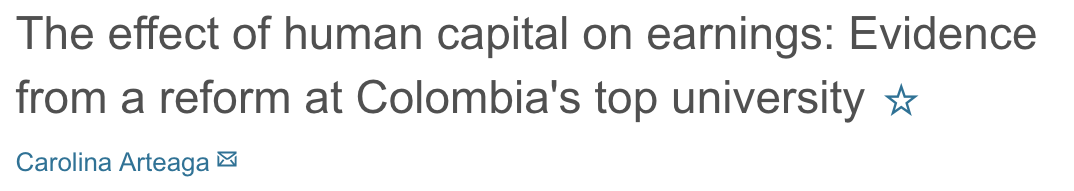
\includegraphics[width=10cm]{/Users/florianhollenbach/Documents/GitHub/Polisci209_2018/slides/week2/uni1.png}
\end{center}

\begin{center}
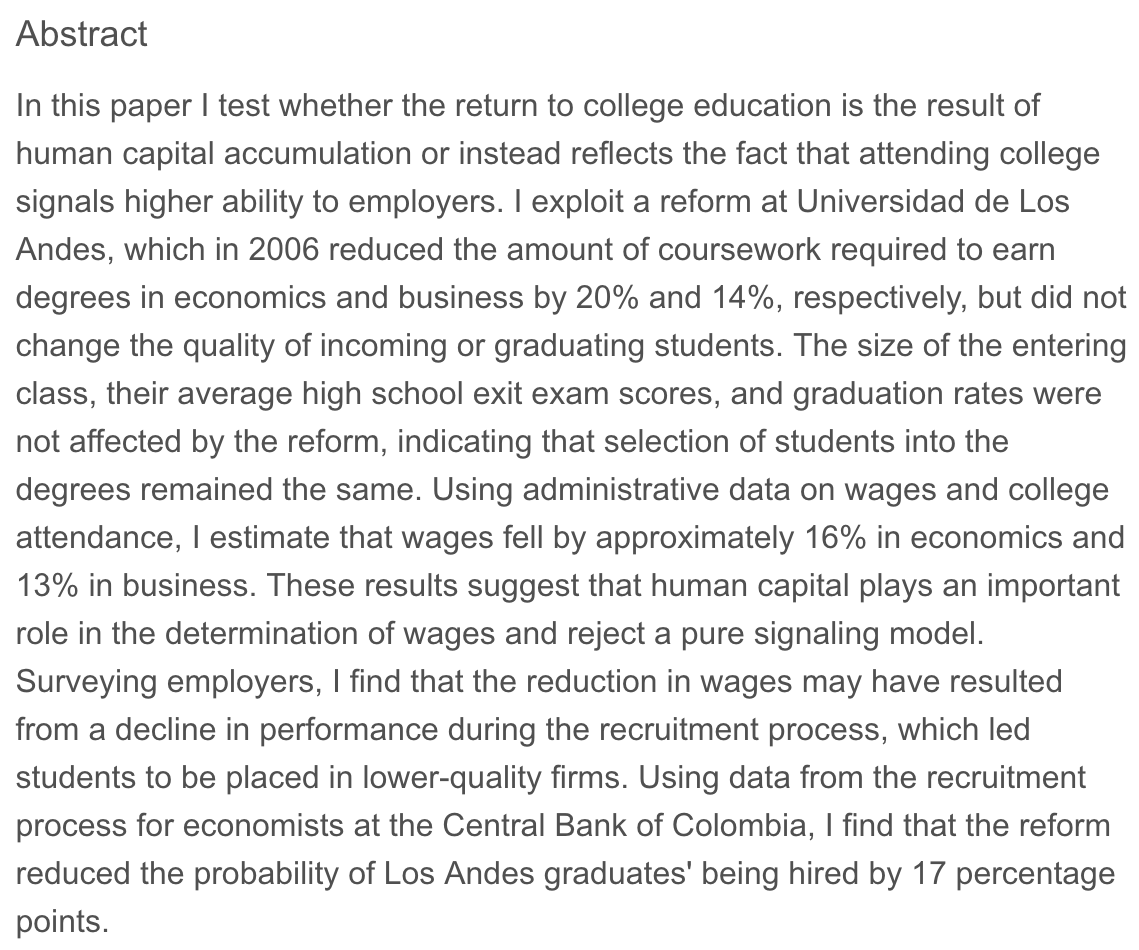
\includegraphics[width=5cm]{/Users/florianhollenbach/Documents/GitHub/Polisci209_2018/slides/week2/uni2.png}
\end{center}
\end{frame}


\begin{frame}[label={sec:org9601c6b}]{Fundamental Problem of Causal Inference}
\begin{center}
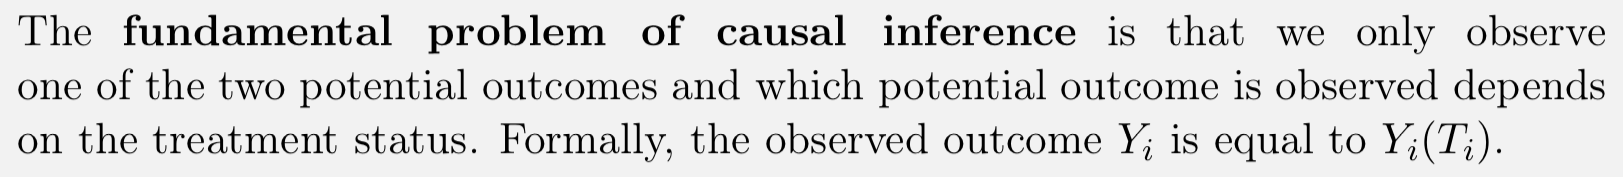
\includegraphics[width=10cm]{/Users/florianhollenbach/Documents/GitHub/Polisci209_2018/slides/week2/fpci.png}
\end{center}
\end{frame}


\begin{frame}[label={sec:orgbaedf58}]{How can we estimate the causal effect?}
\begin{itemize}
\item We try to estimate the \emph{average causal effect} in our sample (SATE) by comparing groups
\item In our sample, does the \emph{Treatment} on average cause a change in \emph{Y}?
\end{itemize}
\pause
\begin{center}
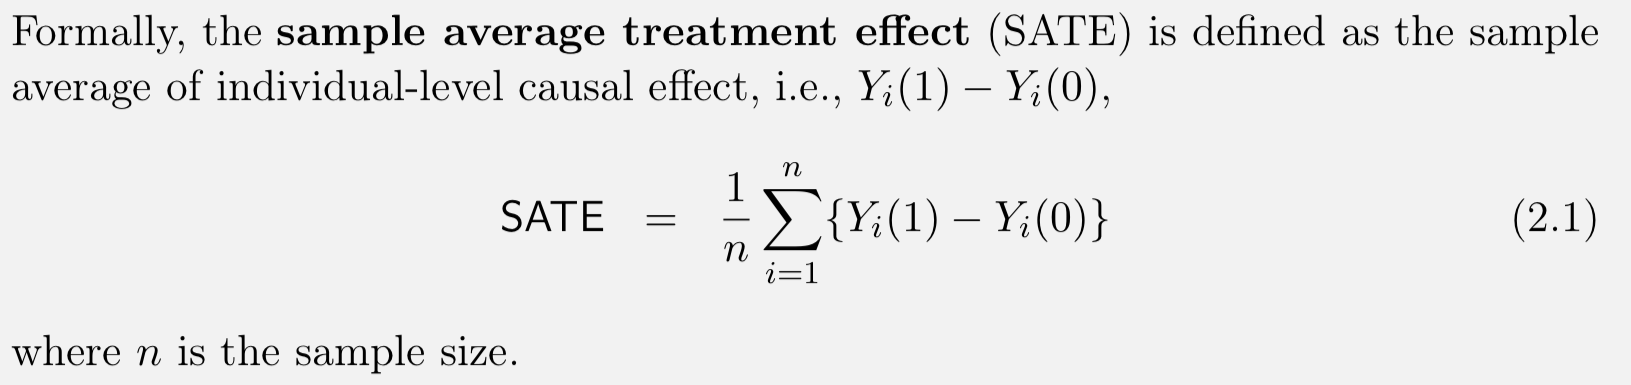
\includegraphics[width=10cm]{/Users/florianhollenbach/Documents/GitHub/Polisci209_2018/slides/week2/sate.png}
\end{center}
But again we only observe one outcome per person!
\end{frame}

\begin{frame}[label={sec:orge4d7524}]{How can we find the causal effect?}
Solution: We compare the average of those who received the treatment (\emph{treated group}) to the average of those who did not (\emph{control group})
\pause


Is this enough?

\pause
Are the two groups comparable?
\end{frame}


\begin{frame}[label={sec:org1fe48df}]{Experiments/Randomized Control Trials}
\begin{itemize}
\item In \emph{Randomized Control Trials} the researcher assigns \emph{treatment} and \emph{control} group status
\end{itemize}
\pause
\begin{itemize}
\item By randomizing the assignment, we guarantee that the two groups are comparable (on average the same) in all other dimensions
\item The random assignment \emph{balances} out treatment and control group
\end{itemize}
\end{frame}

\begin{frame}[label={sec:org996c645}]{Experiments/Randomized Control Trials}
\begin{center}
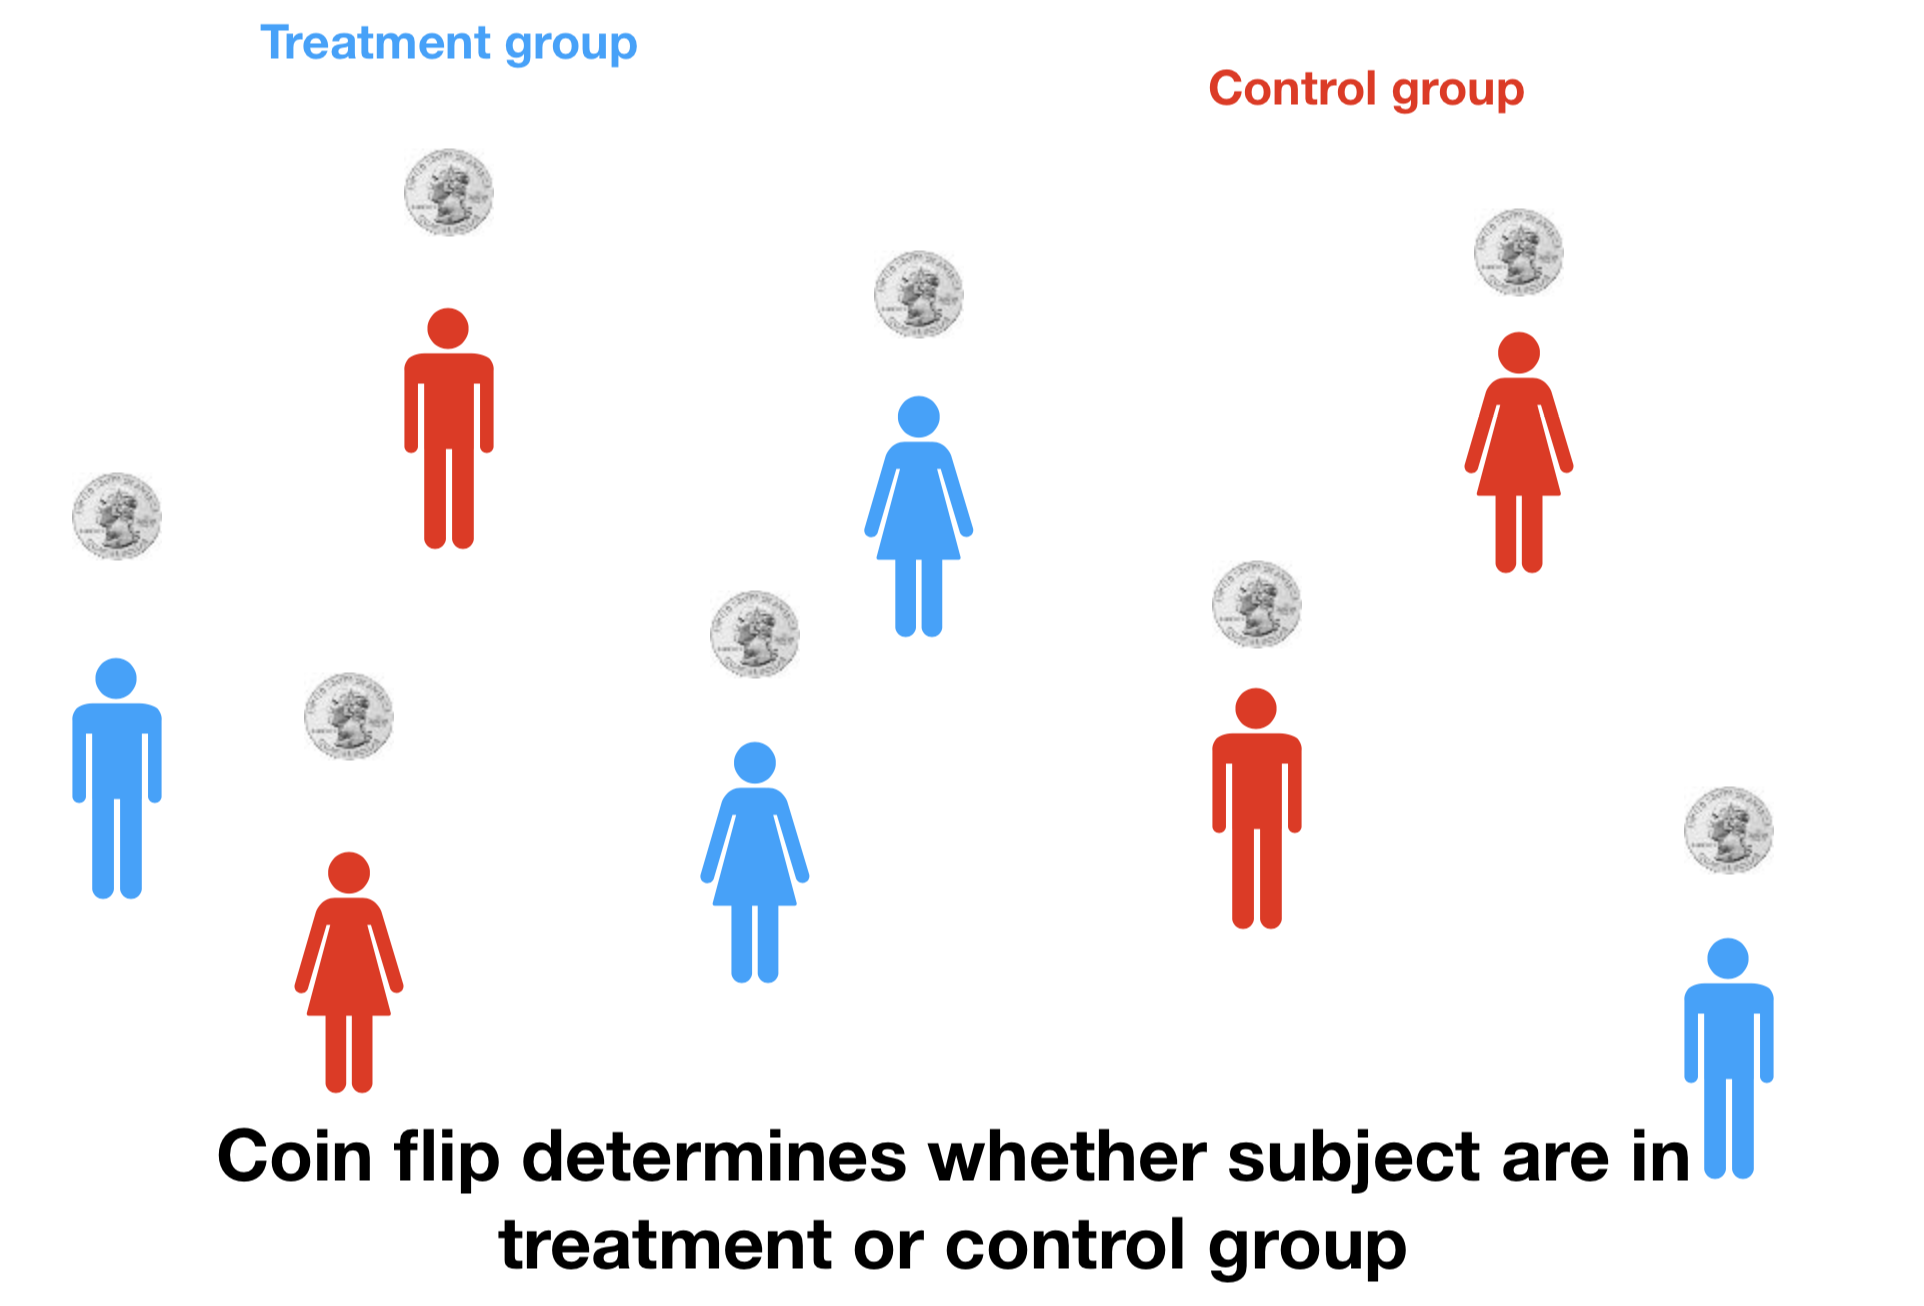
\includegraphics[width=10cm]{/Users/florianhollenbach/Documents/GitHub/Polisci209_2018/slides/week2/experiment.png}
\end{center}
\end{frame}


\begin{frame}[label={sec:org5a51ae9}]{Experiments/Randomized Control Trials}
\begin{center}
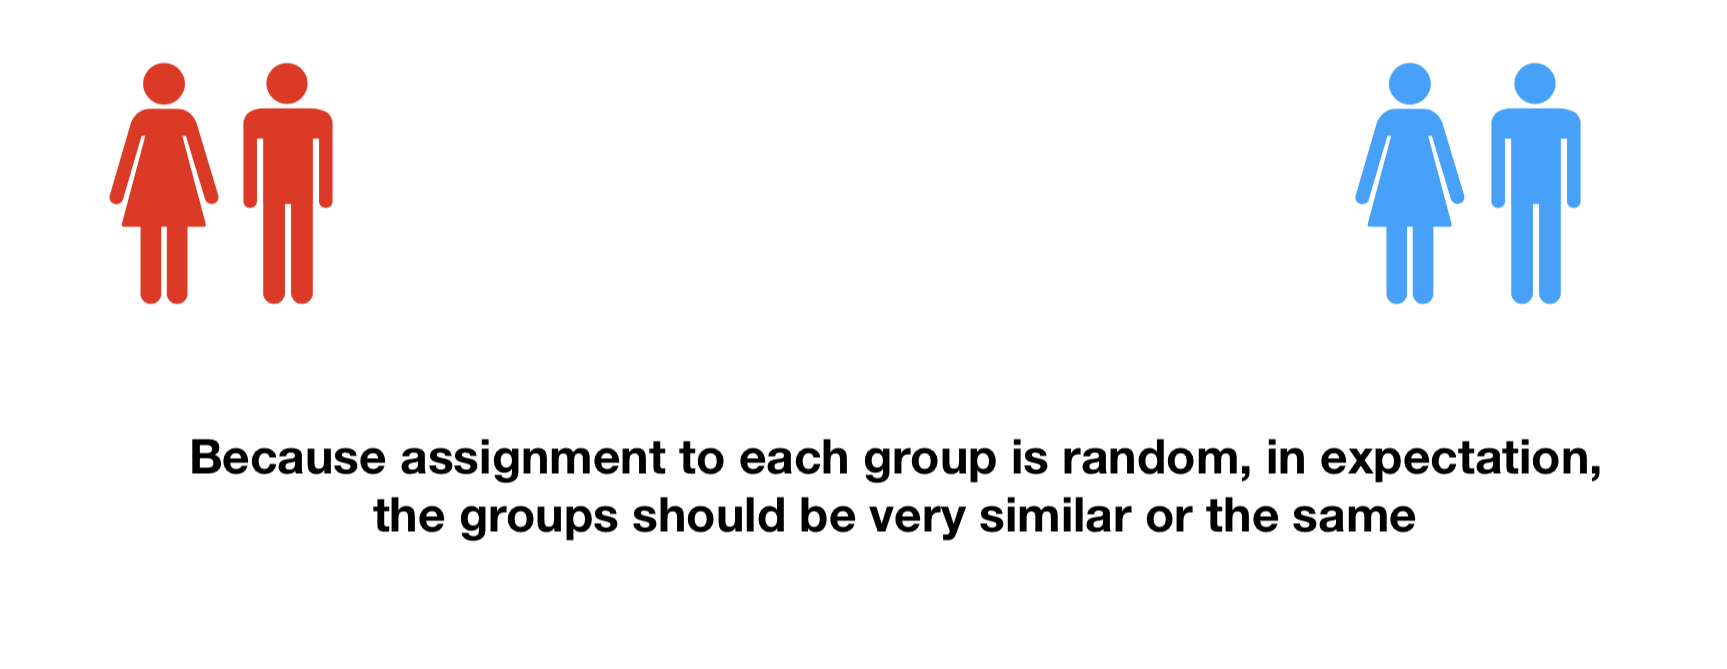
\includegraphics[width=10cm]{/Users/florianhollenbach/Documents/GitHub/Polisci209_2018/slides/week2/experiment3.png}
\end{center}
\end{frame}

\begin{frame}[label={sec:org53343d4}]{Experiments/Randomized Control Trials}
\begin{itemize}
\item On average the two groups are going to be the same on all (pre-treatment) dimensions
\item The difference in the outcome is therefore \emph{caused} by the treatment
\end{itemize}
\end{frame}


\begin{frame}[label={sec:org54befa2}]{Experiments/Randomized Control Trials}
\begin{center}
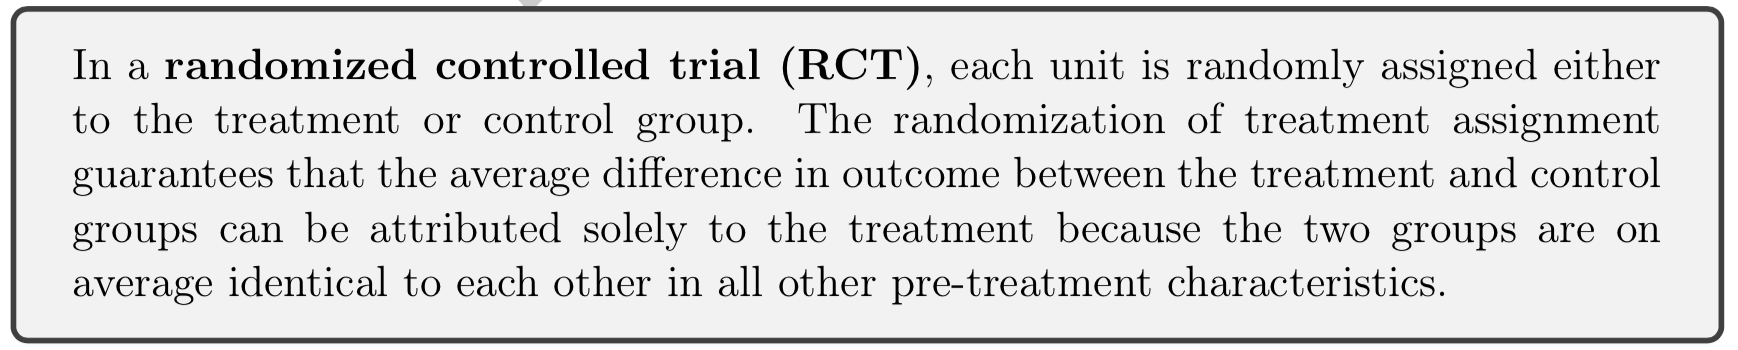
\includegraphics[width=10cm]{/Users/florianhollenbach/Documents/GitHub/Polisci209_2018/slides/week2/rct.png}
\end{center}
\end{frame}


\begin{frame}[label={sec:org3177bd8}]{Experiments/Randomized Control Trials}
\Large{Internal validity vs external validity}
\end{frame}


\begin{frame}[label={sec:org653865f}]{Experiments/Randomized Control Trials}
\begin{itemize}
\item People may behave differently because they are observed (\emph{Hawthorne effect})
\item People may behave differently because they expect the \emph{treatment} to work (\emph{placebo effect})
\end{itemize}
\end{frame}

\begin{frame}[label={sec:org81eb5fc}]{Experiment on Exclusionary Attitudes}
Causal Effect of Intergroup Contact on Exclusionary Attitudes -- by Ryan D. Enos
\begin{center}
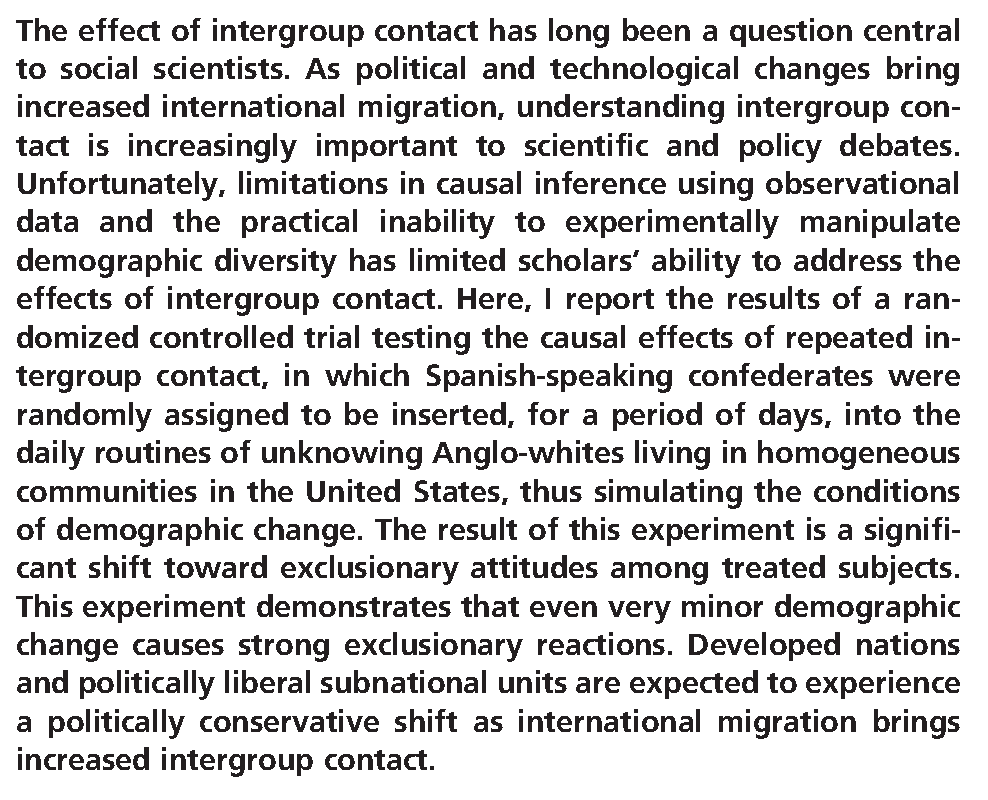
\includegraphics[width=7cm]{/Users/florianhollenbach/Documents/GitHub/Polisci209_2018/slides/week2/exclusion_experiment1.pdf}
\end{center}
\end{frame}

\begin{frame}[label={sec:org77aecc9}]{Experiment on Exclusionary Attitudes}
\begin{center}
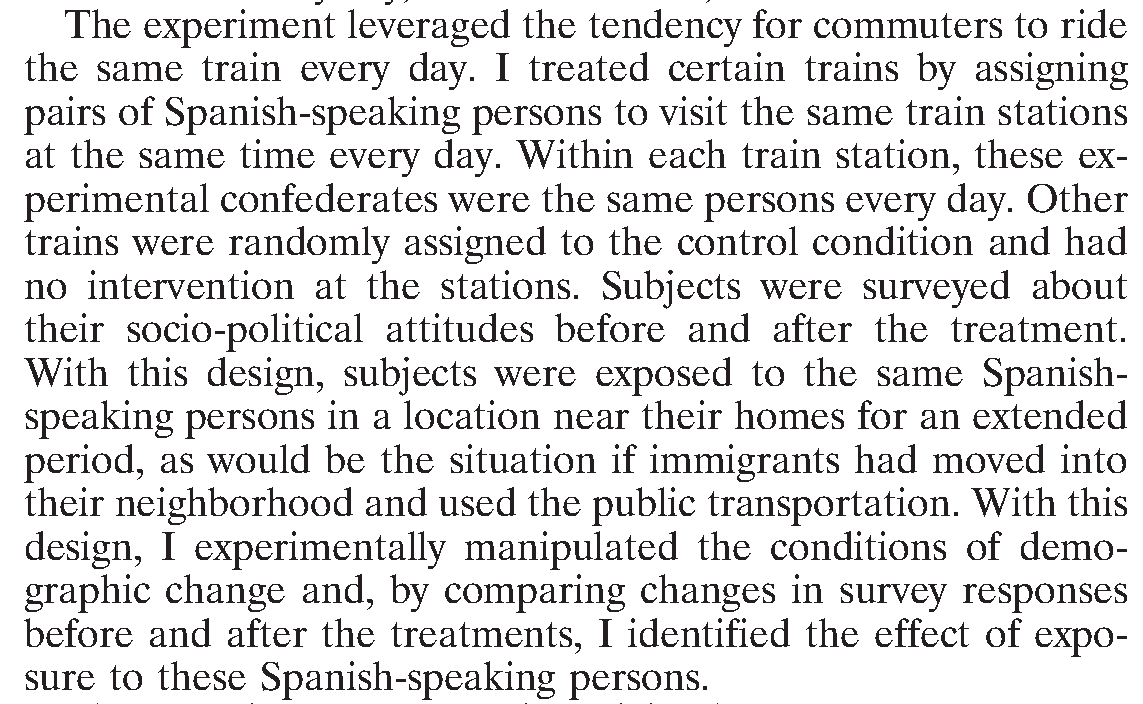
\includegraphics[width=8cm]{/Users/florianhollenbach/Documents/GitHub/Polisci209_2018/slides/week2/exclusion_experiment2.pdf}
\end{center}
\end{frame}


\begin{frame}[label={sec:org0f6ed4a}]{Experiment on Exclusionary Attitudes}
\begin{center}
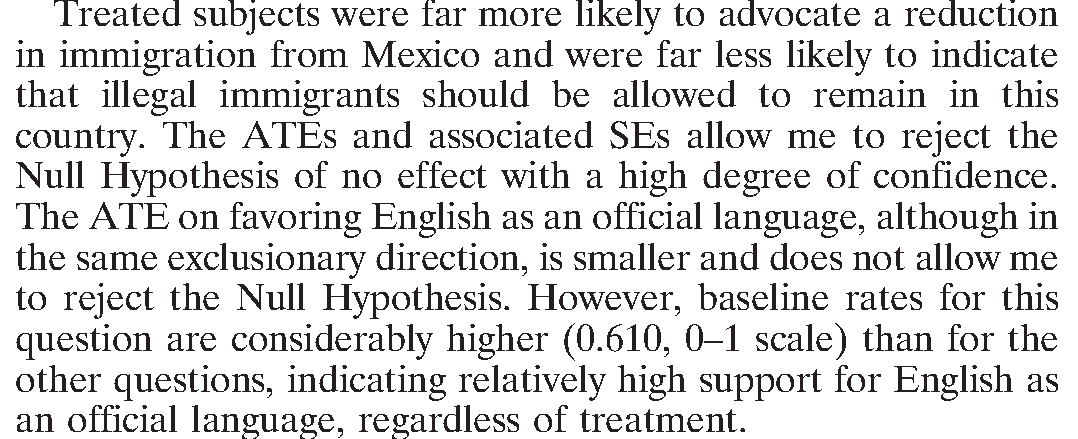
\includegraphics[width=8cm]{/Users/florianhollenbach/Documents/GitHub/Polisci209_2018/slides/week2/exclusion_experiment3.pdf}
\end{center}
\end{frame}


\begin{frame}[label={sec:org0307523}]{Experiment on Exclusionary Attitudes}
\LARGE{Let's look at the data!}
\end{frame}
\end{document}